\documentclass[14pt,a4paper]{extarticle}

\usepackage{iftex}
\ifPDFTeX
  \usepackage[T2A]{fontenc}
  \usepackage[utf8]{inputenc}
  \usepackage[english,russian]{babel}
  \IfFileExists{tempora.sty}{\usepackage{tempora}}{}
\else
  \usepackage{fontspec}
  \IfFontExistsTF{Times New Roman}{\setmainfont{Times New Roman}}{%
    \IfFontExistsTF{Liberation Serif}{\setmainfont{Liberation Serif}}{\setmainfont{CMU Serif}}}
  \usepackage[english,russian]{babel}
\fi

\usepackage[left=30mm,right=15mm,top=20mm,bottom=20mm]{geometry}
\usepackage{setspace}
\onehalfspacing
\setlength{\parindent}{1.25cm}
\usepackage{indentfirst}
\usepackage{graphicx}
\usepackage{float}
\usepackage{pdflscape}
\usepackage{needspace}
\usepackage{array}
\usepackage{xltabular}
\usepackage{booktabs}
\usepackage{enumitem}
\setlist{nosep,leftmargin=*,labelindent=\parindent}
\usepackage[labelsep=endash,font=small]{caption}
\usepackage{titlesec}
\titleformat{\section}{\normalfont\large\bfseries}{\thesection}{1em}{}
\titleformat{\subsection}{\normalfont\normalsize\bfseries}{\thesubsection}{1em}{}
\usepackage[hidelinks]{hyperref}

\renewcommand{\arraystretch}{1.15}
\newcolumntype{L}{>{\raggedright\arraybackslash}X}

\renewcommand{\_}{\textunderscore\allowbreak}
\newcommand{\teacher}{Тюрин И. Н.}

\begin{document}

\begin{titlepage}
  \centering
  \vspace*{5mm}
  Федеральное государственное автономное образовательное учреждение\\
  высшего образования «Национальный исследовательский университет\\
  ИТМО»\par
  \vspace{4mm}
  \textit{Факультет программной инженерии и компьютерной техники}\\
  \textit{Направление подготовки: 09.03.04 -- Программная инженерия, Системное}\\
  \textit{и прикладное программное обеспечение}\par
  \vspace{18mm}
  Дисциплина: Информационные системы\par
  \vspace{30mm}
  {\large\bfseries Курсовая работа. Этап 2\par}
  \vspace{1mm}
  {\large Информационная система студии сайкл-тренировок\par}
  \vfill
  \begin{flushright}
    Выполнил:\\
    Гришин Артем Евгеньевич\\
    Группа: Р3311\\[3mm]
    Проверил:\\
    \teacher
  \end{flushright}
  \vspace{25mm}
  г. Санкт-Петербург, 2026\par
\end{titlepage}

\tableofcontents
\newpage

\section{Даталогическая модель}

По сравнению с ER-моделью в даталогической модели у абонемента добавлен внешний ключ \texttt{issued\_by} --- администратор, выдавший абонемент без оплаты. Также добавлена одна таблица --- \texttt{training\_trainer}. Связь «многие-ко-многим» «ведёт» между Тренером и Занятием в реляционной базе данных реализуется через отдельную таблицу с составным первичным ключом (\texttt{training\_id}, \texttt{trainer\_id}). В этой же таблице хранится роль тренера на занятии (\texttt{role}: \texttt{LEAD} или \texttt{ASSISTANT}).

Ограничения для нескольких тренеров на занятии:
\begin{itemize}
  \item ведущий на занятии не больше одного --- частичный уникальный индекс \texttt{UNIQUE (training\_id) WHERE role = 'LEAD'};
  \item ведущий на занятии есть всегда --- отложенный триггер;
  \item тренер не назначается на два занятия, пересекающихся по времени, --- триггер на \texttt{training\_trainer} и \texttt{training};
  \item на занятие назначается только работающий тренер (\texttt{trainer.is\_active}) --- триггер на \texttt{training\_trainer}.
\end{itemize}

\begin{landscape}
\begin{figure}[p]
  \centering
  \IfFileExists{diagrams/datalogical-model.png}{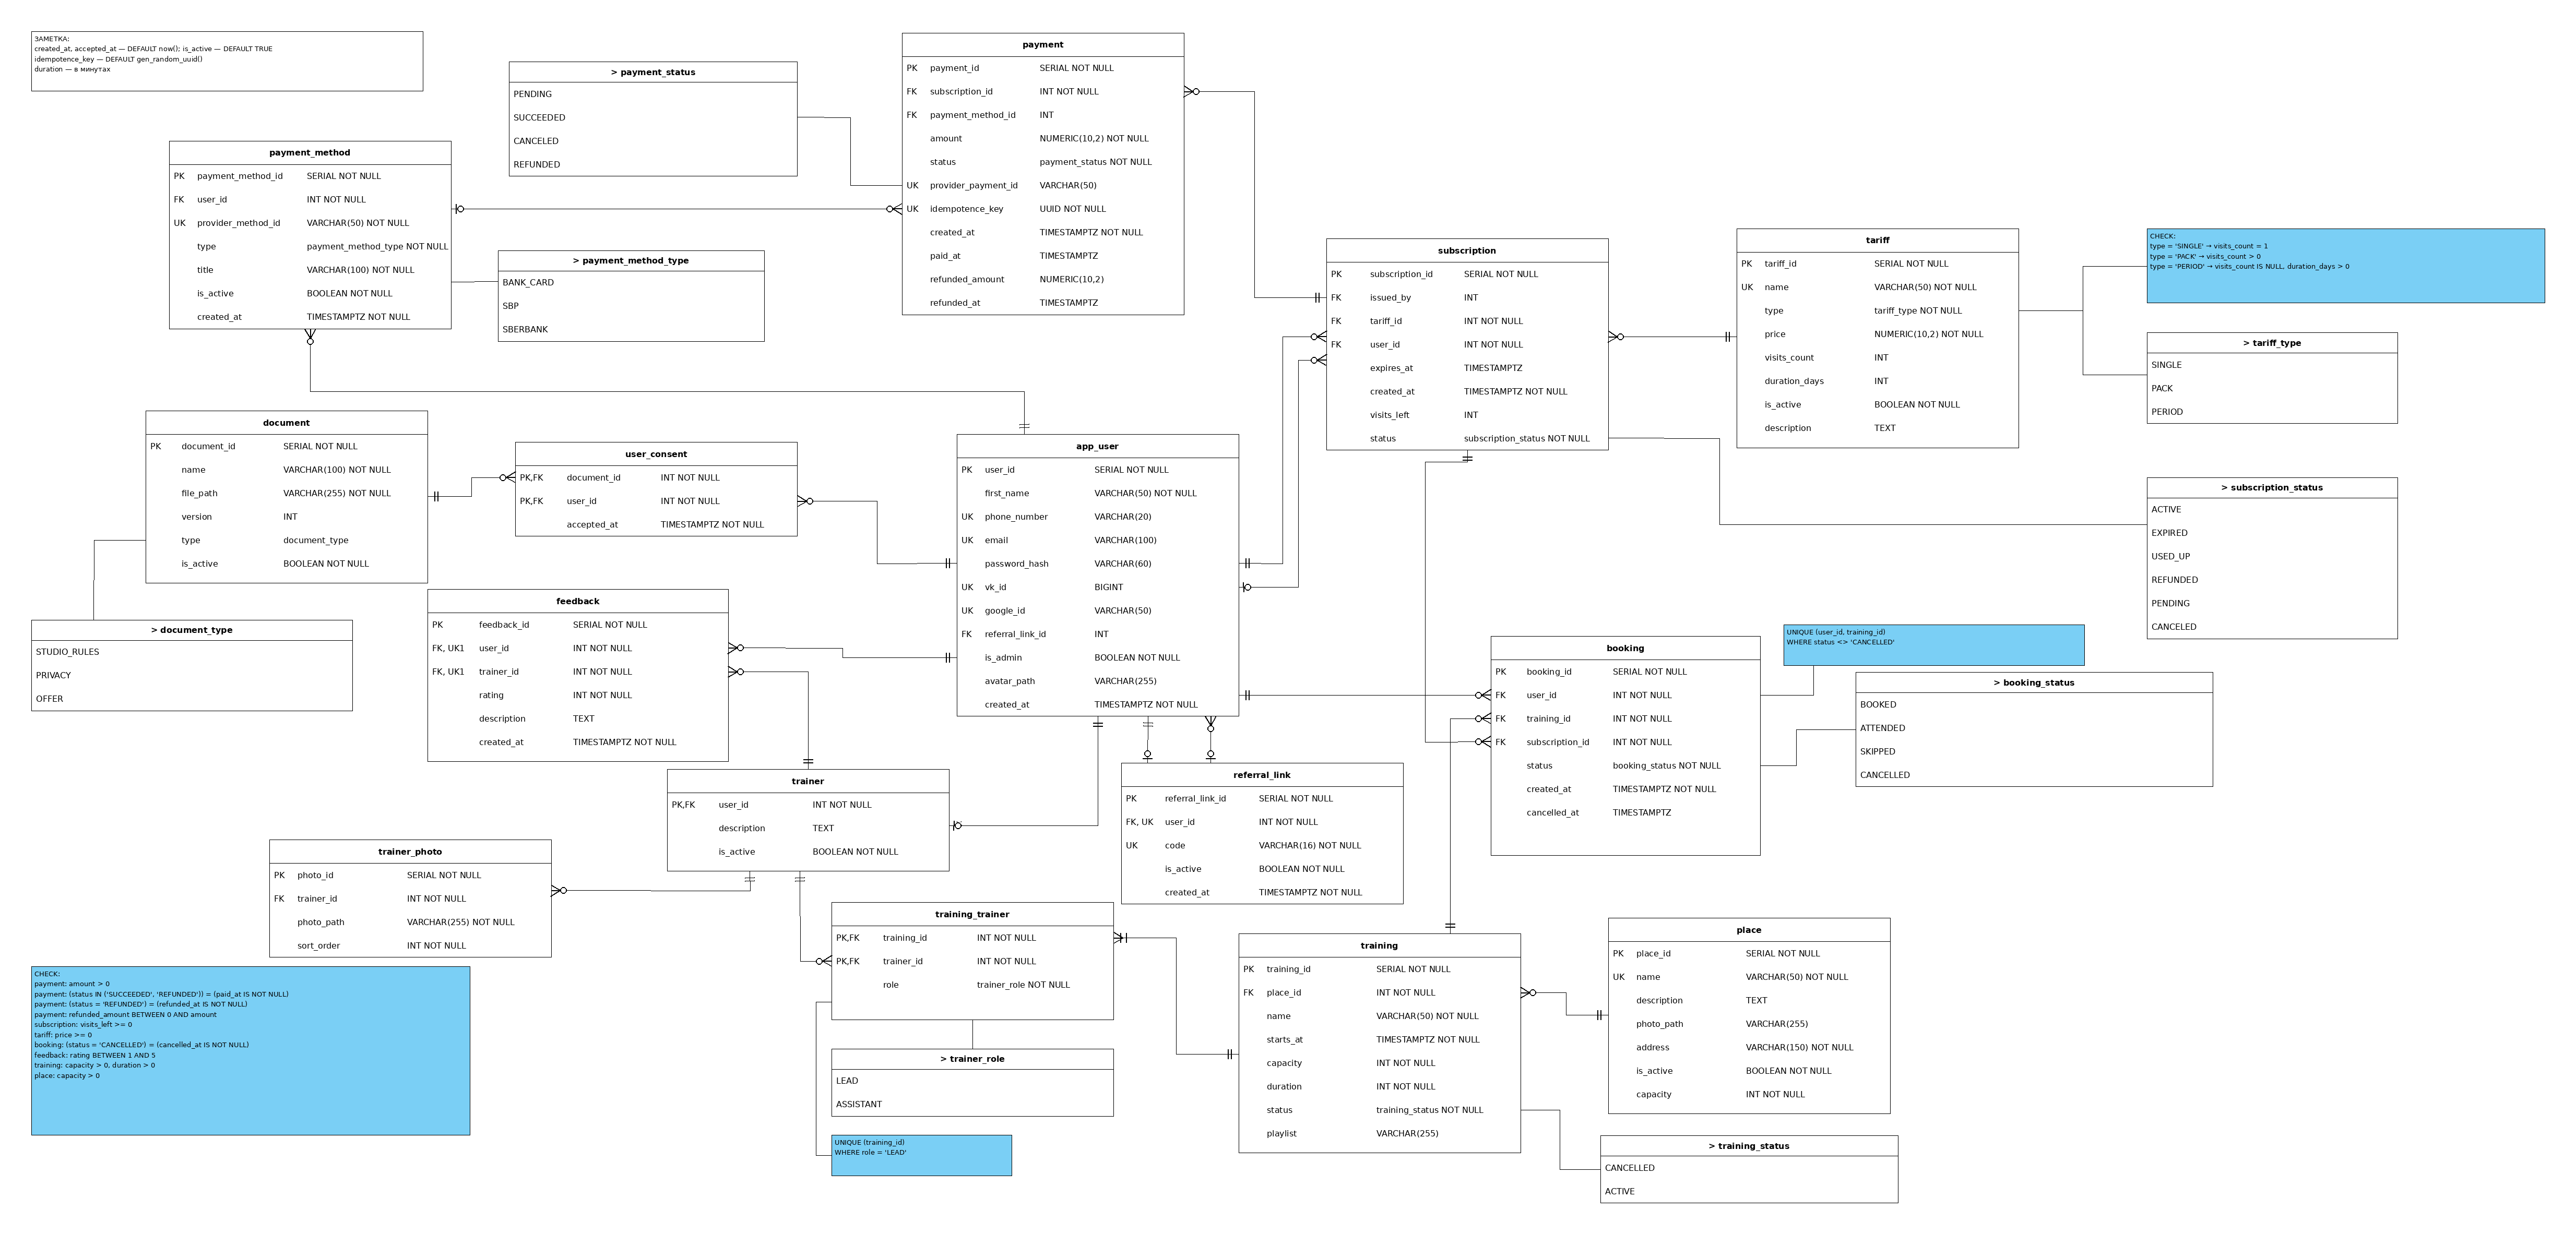
\includegraphics[width=\linewidth,height=0.9\textheight,keepaspectratio]{diagrams/datalogical-model.png}}{\includegraphics[width=\linewidth,height=0.9\textheight,keepaspectratio]{datalogical-model.png}}
  \caption{Даталогическая модель}
  \label{fig:dl}
\end{figure}
\end{landscape}

\sloppy
\section{Реализация в PostgreSQL}

База данных реализована в PostgreSQL 16. Скрипты лежат в каталоге \texttt{sql} репозитория и выполняются в таком порядке:

\begingroup\small
\begin{xltabular}{\textwidth}{|p{3.4cm}|L|}
  \hline
  \textbf{Файл} & \textbf{Содержание} \\ \hline
  \endhead
  \texttt{create.sql} & Перечисляемые типы, таблицы, первичные и внешние ключи, ограничения \texttt{UNIQUE}, \texttt{CHECK}, \texttt{NOT NULL}, \texttt{DEFAULT}, частичные уникальные индексы. \\ \hline
  \texttt{triggers.sql} & Триггерные функции и триггеры. \\ \hline
  \texttt{functions.sql} & Функции и процедуры для прецедентов, представления для статистики. \\ \hline
  \texttt{indexes.sql} & Индексы. \\ \hline
  \texttt{fill.sql} & Тестовые данные. \\ \hline
  \texttt{drop.sql} & Удаление всех объектов базы данных. \\ \hline
  \texttt{explain.sql} & Планы запросов для обоснования индексов. \\ \hline
\end{xltabular}
\endgroup

Тестовые данные минимальные, но покрывают все таблицы и статусы: 3 места проведения (одно закрыто), 5 тарифов (один снят с продажи), 4 документа (одна старая редакция правил), 5 тренеров (один не работает, один также администратор), 22 клиента, 28 занятий на неделе вокруг текущей даты (одно отменено), 29 абонементов, 27 платежей, 88 записей, 16 отзывов. Записи на прошедшие занятия отмечены как «пришёл» или «не пришёл», часть записей отменена рано и поздно. Через функции выполнены регистрация по реферальной ссылке с покупкой пакета и наградой пригласившему, неоплаченная покупка, выдача абонемента администратором и частичный возврат платежа. Все данные проходят через триггеры, поэтому скрипт заполнения одновременно проверяет их работу.

\subsection{Ограничения целостности средствами DDL}

\begin{itemize}
  \item Первичные и внешние ключи всех таблиц. При удалении пользователя удаляются его согласия и реферальная ссылка, при удалении тренера --- его фотографии, при удалении занятия --- назначения тренеров; остальные внешние ключи запрещают удаление связанных строк.
  \item \texttt{UNIQUE}: телефон, почта, VK ID и Google ID пользователя; код реферальной ссылки и её владелец; название тарифа и места проведения; токен способа оплаты; идентификатор платежа в платёжном сервисе и ключ идемпотентности; пара (клиент, тренер) в отзыве.
  \item Частичные уникальные индексы:
  \begin{itemize}
    \item \texttt{booking (user\_id, training\_id) WHERE status <> 'CANCELLED'} --- клиент не записан на занятие дважды, но после отмены может записаться снова;
    \item \texttt{training\_trainer (training\_id) WHERE role = 'LEAD'} --- не больше одного ведущего;
    \item \texttt{payment (subscription\_id) WHERE status = 'PENDING'} --- не больше одного неоплаченного платежа за абонемент, повторное нажатие «Купить» не создаёт второй платёж;
    \item \texttt{payment (subscription\_id) WHERE status IN ('SUCCEEDED', 'REFUNDED')} --- абонемент оплачивается только один раз.
  \end{itemize}
  \item \texttt{CHECK}:
  \begin{itemize}
    \item у пользователя есть хотя бы один способ входа: телефон, почта, VK ID или Google ID; пароль задаётся только вместе с телефоном или почтой;
    \item вид тарифа согласован с числом занятий и сроком: разовое --- одно занятие, пакет --- больше нуля занятий, абонемент на период --- без ограничения занятий, срок задан; цена не отрицательна, срок положителен;
    \item остаток занятий абонемента не отрицателен;
    \item сумма платежа положительна; дата оплаты есть только у оплаченного или возвращённого платежа; сумма и дата возврата есть только у возвращённого; сумма возврата не больше суммы платежа;
    \item время отмены есть только у отменённой записи;
    \item оценка в отзыве от 1 до 5, тренер не оставляет отзыв о себе;
    \item вместимость и продолжительность занятия, вместимость места проведения положительны; номер редакции документа и порядок фотографии не отрицательны.
  \end{itemize}
\end{itemize}

\subsection{Триггеры}

Ограничения, которые затрагивают несколько таблиц, реализованы триггерами. При одновременных запросах триггеры блокируют строку занятия или тренера (\texttt{SELECT \ldots{} FOR UPDATE}), поэтому две транзакции не займут последнее место и не назначат тренера на два занятия одновременно.

\begingroup\small
\begin{xltabular}{\textwidth}{|p{4.4cm}|p{3.4cm}|L|}
  \hline
  \textbf{Триггер} & \textbf{Таблица, событие} & \textbf{Что проверяет или делает} \\ \hline
  \endhead
  \texttt{training\_lead\_required}, \texttt{training\_trainer\_lead\_required} & \texttt{training}: INSERT; \texttt{training\_trainer}: UPDATE, DELETE & У занятия есть ведущий тренер. Триггеры отложенные (\texttt{DEFERRABLE INITIALLY DEFERRED}): проверка выполняется при фиксации транзакции, поэтому занятие и его тренеры добавляются в одной транзакции. \\ \hline
  \texttt{training\_trainer\_check} & \texttt{training\_trainer}: INSERT, UPDATE & Тренер работает в студии и не ведёт другое занятие, пересекающееся по времени. \\ \hline
  \texttt{training\_check} & \texttt{training}: INSERT, UPDATE & Место проведения открыто; вместимость занятия не больше вместимости места и не меньше числа записанных; отменённое занятие не изменяется. \\ \hline
  \texttt{training\_after\_update} & \texttt{training}: UPDATE & При отмене занятия отменяет все записи на него. При изменении времени или продолжительности проверяет, что у тренеров нет пересечений. \\ \hline
  \texttt{booking\_insert} & \texttt{booking}: INSERT & Занятие не отменено; абонемент принадлежит тому же клиенту, действует и не заканчивается до начала занятия; есть свободное место. Списывает одно занятие с абонемента (у безлимитного остаток не ведётся). \\ \hline
  \texttt{booking\_update} & \texttt{booking}: UPDATE & Клиент, занятие и абонемент записи не меняются; допустимы переходы статуса «записан» $\to$ «пришёл», «не пришёл», «отменена» и «пришёл» $\leftrightarrow$ «не пришёл». При отмене не позднее чем за 24 часа до начала или при отмене занятия возвращает занятие на абонемент. \\ \hline
  \texttt{subscription\_check} & \texttt{subscription}: INSERT, UPDATE & Владелец и тариф не меняются; абонемент без оплаты выдаёт только администратор. Переводит абонемент в статус «использован», когда остаток стал нулём, и обратно в «действует» (или «истёк»), когда занятие вернулось. \\ \hline
  \texttt{payment\_check} & \texttt{payment}: INSERT, UPDATE & Способ оплаты принадлежит владельцу абонемента и не удалён. \\ \hline
  \texttt{feedback\_check} & \texttt{feedback}: INSERT, UPDATE & Отзыв оставляет клиент, который посетил занятие этого тренера. \\ \hline
\end{xltabular}
\endgroup

На рис.~\ref{fig:booking} показано, как при записи на занятие проверки распределены между функцией и триггерами. Все шаги выполняются в одной транзакции: если любая проверка не прошла, запись не создаётся и занятие с абонемента не списывается.

\begin{figure}[H]
  \centering
  \IfFileExists{diagrams/booking-flow.png}{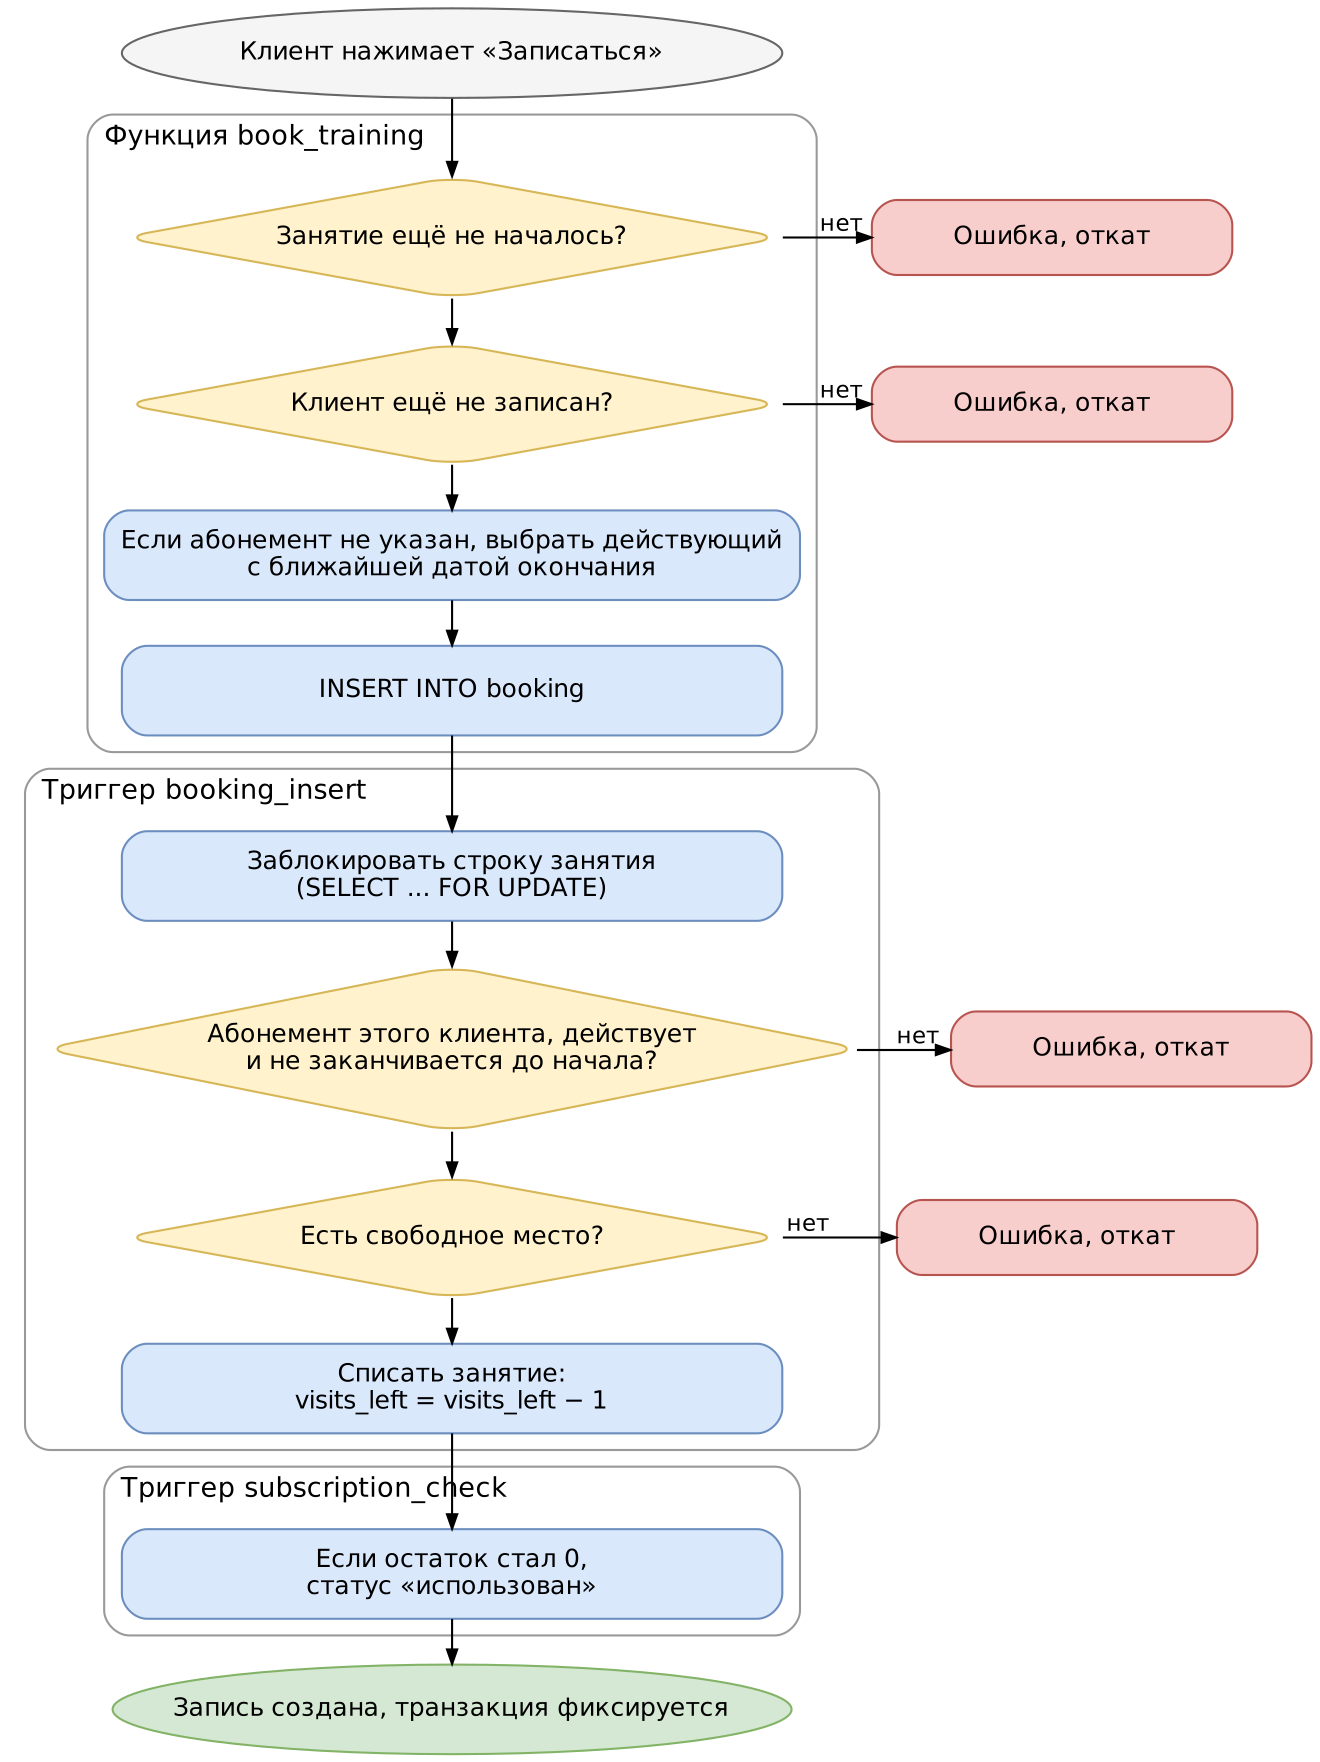
\includegraphics[width=0.78\textwidth]{diagrams/booking-flow.png}}{\includegraphics[width=0.78\textwidth]{booking-flow.png}}
  \caption{Запись на занятие: функция и триггеры}
  \label{fig:booking}
\end{figure}

\section{Функции и процедуры}

Функции выполняют прецеденты целиком в одной транзакции: проверяют права и бизнес-правила, которые зависят от текущего времени, и изменяют данные. Ограничения целостности при этом остаются в триггерах, поэтому действуют и при изменении данных в обход функций.

\begingroup\small
\begin{xltabular}{\textwidth}{|p{4.6cm}|p{3.6cm}|L|}
  \hline
  \textbf{Функция} & \textbf{Прецедент} & \textbf{Что делает} \\ \hline
  \endhead
  \texttt{register\_user} & Регистрация & Проверяет согласие со всеми действующими документами, создаёт пользователя, реферальную ссылку и согласия; привязывает приглашение, если код ссылки действителен. Возвращает ID пользователя. \\ \hline
  \texttt{get\_schedule} & Запись на занятие & Расписание за период с фильтром по месту и тренеру: занятие, место, ведущий, число свободных мест. \\ \hline
  \texttt{book\_training} & Запись на занятие & Проверяет, что занятие ещё не началось и клиент не записан. Если абонемент не указан, выбирает действующий абонемент с ближайшей датой окончания. Создаёт запись. \\ \hline
  \texttt{cancel\_booking} & Отмена записи & Проверяет владельца записи и что занятие не началось, отменяет запись. Возвращает, вернулось ли занятие на абонемент. \\ \hline
  \texttt{buy\_tariff} & Покупка абонемента & Проверяет, что тариф в продаже, оформляет абонемент «ожидает оплаты» и платёж на цену тарифа. Повторный вызов возвращает тот же абонемент и платёж. \\ \hline
  \texttt{create\_payment} & Покупка абонемента & Повторная оплата неоплаченного абонемента: возвращает текущий неоплаченный платёж или создаёт новый. \\ \hline
  \texttt{confirm\_payment} & Покупка абонемента & Переводит платёж в «оплачен», абонемент в «действует» и задаёт дату окончания. Если это первая оплата приглашённого клиента, выдаёт пригласившему разовое занятие. Повторный вызов ничего не меняет. \\ \hline
  \texttt{cancel\_payment} & Покупка абонемента & Отменяет неоплаченный платёж, абонемент остаётся «ожидает оплаты». \\ \hline
  \texttt{refund\_payment} & Возврат платежа & Проверяет сумму возврата, отменяет будущие записи по абонементу, переводит платёж и абонемент в «возвращён». \\ \hline
  \texttt{grant\_subscription} & Выдача абонемента без оплаты & Создаёт действующий абонемент с указанием выдавшего администратора. \\ \hline
  \texttt{create\_training} & Управление своими занятиями & Создаёт занятие, ведущего и ассистентов в одной транзакции. \\ \hline
  \texttt{update\_training} & Управление своими занятиями & Проверяет, что изменяет ведущий и занятие не началось, изменяет переданные поля. \\ \hline
  \texttt{cancel\_training} & Управление своими занятиями & Проверяет, что отменяет ведущий, отменяет занятие; записи отменяются триггером с возвратом занятий. \\ \hline
  \texttt{mark\_attendance} & Отметка посещения & Проверяет, что отмечает тренер этого занятия или администратор и занятие началось, ставит «пришёл» или «не пришёл». \\ \hline
  \texttt{save\_feedback} & Отзыв о тренере & Создаёт отзыв или изменяет существующий. \\ \hline
  \texttt{expire\_subscriptions} (процедура) & --- & Переводит абонементы с прошедшей датой окончания в статус «истёк». Вызывается приложением по расписанию. \\ \hline
\end{xltabular}
\endgroup

Для статистики созданы представления: \texttt{training\_load} --- число записанных и пришедших и загрузка каждого занятия в процентах, \texttt{trainer\_rating} --- средняя оценка и число отзывов тренера, \texttt{revenue\_by\_month} --- выручка за вычетом возвратов по месяцам и тарифам.

\section{Индексы}

PostgreSQL сам создаёт индексы для первичных ключей и ограничений \texttt{UNIQUE}. Поэтому уже есть индексы для входа по телефону, почте, VK ID и Google ID, для поиска платежа по уведомлению платёжного сервиса и для проверки повторной записи. Дополнительные индексы выбраны по запросам прецедентов:

\begingroup\small
\begin{xltabular}{\textwidth}{|p{5.4cm}|L|}
  \hline
  \textbf{Индекс} & \textbf{Запрос и прецедент} \\ \hline
  \endhead
  \texttt{training (starts\_at) WHERE status = 'ACTIVE'} & Расписание за период (запись на занятие). Отменённые занятия в расписании не показываются, поэтому в индекс не входят. \\ \hline
  \texttt{training USING gist (training\_period(starts\_at, duration)) WHERE status = 'ACTIVE'} & Поиск занятий, пересекающихся по времени, в триггере при назначении тренера (управление своими занятиями). \\ \hline
  \texttt{booking (training\_id) WHERE status <> 'CANCELLED'} & Подсчёт занятых мест в расписании и в триггере записи, список записавшихся (отметка посещения), отмена записей при отмене занятия. \\ \hline
  \texttt{booking (user\_id)} & Записи клиента в личном кабинете. \\ \hline
  \texttt{subscription (user\_id)} & Выбор абонемента при записи, абонементы клиента в личном кабинете. \\ \hline
  \texttt{payment (subscription\_id)} & История платежей клиента, поиск платежа для возврата. \\ \hline
\end{xltabular}
\endgroup

Тестовых данных слишком мало, чтобы планировщик выбирал индексы: на десятках строк полный просмотр таблицы дешевле. Поэтому скрипт \texttt{explain.sql} в отдельной транзакции добавляет данные студии за год (1500 клиентов, около 2900 занятий, 3900 абонементов и платежей, 37\,000 записей), выполняет \texttt{EXPLAIN ANALYZE} запросов сначала с индексами, затем после их удаления, и откатывает транзакцию. Время выполнения запросов:

\begingroup\small
\begin{xltabular}{\textwidth}{|L|>{\centering\arraybackslash}p{2.6cm}|>{\centering\arraybackslash}p{2.6cm}|}
  \hline
  \textbf{Запрос} & \textbf{Без индекса, мс} & \textbf{С индексом, мс} \\ \hline
  \endhead
  Расписание на неделю со свободными местами & 116,5 & 0,25 \\ \hline
  Пересечение занятий тренера по времени & 2,7 & 0,09 \\ \hline
  Список записавшихся на занятие & 2,4 & 0,34 \\ \hline
  Записи клиента & 2,3 & 0,61 \\ \hline
  Действующие абонементы клиента & 0,31 & 0,01 \\ \hline
  История платежей клиента & 0,84 & 0,02 \\ \hline
\end{xltabular}
\endgroup

Без индексов в планах выполняются полные просмотры таблиц, время которых растёт с числом занятий и записей; с индексами просматриваются только нужные строки. Самый большой выигрыш у расписания: без индексов для каждого занятия подсчёт свободных мест просматривает всю таблицу записей.

Индексы по \texttt{trainer\_id} в \texttt{training\_trainer} и \texttt{feedback} не созданы: тренеров в студии несколько человек, на одного приходится заметная доля строк, поэтому планировщик выбирает полный просмотр таблицы.

\end{document}
